\documentclass[11pt, oneside]{article} 
\usepackage{geometry}
\geometry{letterpaper} 
\usepackage{graphicx}
	
\usepackage{amssymb}
\usepackage{amsmath}
\usepackage{parskip}
\usepackage{color}
\usepackage{hyperref}

\graphicspath{{/Users/telliott_admin/Tex/png/}}
% \begin{center} 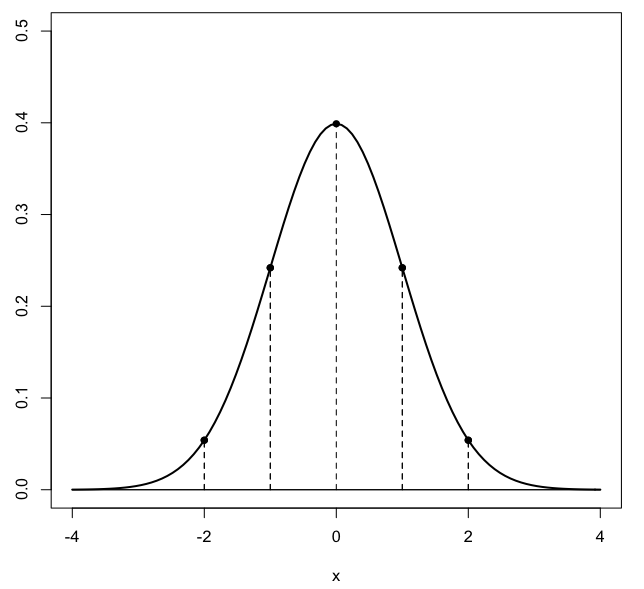
\includegraphics [scale=0.4] {gauss3.png} \end{center}

%break
\title{Headlight problem}
\date{}

\begin{document}
\maketitle
\Large

One of the most interesting properties of the parabola is that any light ray coming down vertically will bounce off the surface of the parabola so that it is reflected to the focus.  Reflecting telescopes are made in this way.  The reverse is also true.  The inside of a headlight has a parabolic shape, so that the light coming out is focused into a parallel beam.

\subsection*{parallel rays are reflected to the focus}
Above we said that if the light source is placed at the focus of a paraboloid headlight, then rays reflected off the surface emerge "straight out" (or up, as we usually draw parabolas).  Conversely, light rays parallel to the axis of symmetry that enter a paraboloid converge at the focus.

Here is a proof of this that uses vectors.  It is not as clean as I'd like (there is a bit of algebra) but it isn't too bad.  Start with a standard parabola centered with its vertex at the origin with equation $y=ax^2$.  At any point on the parabola $P = (x,ax^2)$, the tangent line to the parabola has slope $2ax$, by the most basic result in calculus.

Draw a vector $\mathbf{u}$ from the focus $F = (0,c)$ to the point $P$.  This vector has components

\[ \mathbf{u} = \langle x, ax^2 - c \rangle \]
Draw a vector $\mathbf{v}$ extending vertically up from point $P$, its components are
\[ \mathbf{v} = \langle 0, k \rangle \]
where $k$ can be any constant.
Finally, draw the vector $\mathbf{w}$ parallel to the tangent line.  $\mathbf{w}$ has the same slope as the tangent line, so one version of it could be
\[ \mathbf{w} = \langle 1, 2ax \rangle \]

The statements above about the paths of light rays can be restated as follows:  the angle $\theta$ between $\mathbf{u}$ and $\mathbf{w}$ is equal to the angle $\phi$ between $\mathbf{v}$ and $\mathbf{w}$.  We can calculate these angles using the dot product.  Recall that

\[ \mathbf{u} \cdot \mathbf{w} = u w \cos \theta \]
\[ \mathbf{v} \cdot \mathbf{w} = v w \cos \phi \]

So if $\theta = \phi$, then $\cos \theta = \cos \phi$ and $w \cos \theta = w \cos \phi$ so that
\[ \frac{\mathbf{u} \cdot \mathbf{w}}{u} = \frac{\mathbf{v} \cdot \mathbf{w}}{v} \]
Conversely, if this equality holds, then $\theta = \phi$.

We calculate these values in the usual way:
\[ \mathbf{u} \cdot \mathbf{w} = x + 2ax (ax^2 - c) \]
\[ \mathbf{v} \cdot \mathbf{w} = 2ax k \]
\[ u = | \mathbf{u} | = \sqrt{x^2 + (ax^2 - c)^2} \]
\[ v = | \mathbf{v} | = k \]

Our equation is:
\[ \frac{\mathbf{u} \cdot \mathbf{w}}{u} = \frac{\mathbf{v} \cdot \mathbf{w}}{v} \]
From what we had above, the right-hand side is easy:
\[ \frac{\mathbf{v} \cdot \mathbf{w}}{v} = \frac{2axk}{k} = 2ax \]
We are reassured to see the arbitrary constant $k$ go away.  The left-hand side is a bit of a mess:
\[ \frac{\mathbf{u} \cdot \mathbf{w}}{u}  = \frac{x + 2ax (ax^2 - c)}{\sqrt{x^2 + (ax^2 - c)^2} } \]

So what we need to do is prove that
\[ \frac{x + 2ax (ax^2 - c)}{\sqrt{x^2 + (ax^2 - c)^2} } = 2ax \]
\[ x + 2ax (ax^2 - c) = 2ax \sqrt{x^2 + (ax^2 - c)^2} \]
We can factor out one $x$ right away
\[ 1 + 2a (ax^2 - c) = 2a \sqrt{x^2 + (ax^2 - c)^2} \]
Expand a little bit
\[ 1 + 2a^2x^2 - 2ac = 2a \sqrt{x^2 + (ax^2 - c)^2} \]

And now we just have to do the grunt work of squaring both sides.  The left-hand side is
\[ (1 + 2a^2x^2 - 2ac)^2 \]
\[ = 1 + 2a^2x^2 - 2ac + 2a^2x^2 + 4a^4x^4 - 4a^3cx^2 - 2ac - 4a^3cx^2 + 4a^2c^2 \]
\[ = 1 + 4a^2x^2 - 4ac + 4a^4x^4 - 8a^3cx^2 + 4a^2c^2 \]
while the square of the right-hand side is
\[ 4a^2 \ [ \ x^2 + (ax^2 - c)^2 \ ] \]
\[ = 4a^2(x^2 + a^2x^4 - 2acx^2 + c^2) \]
\[ = 4a^2x^2 + 4a^4x^4 - 8a^3cx^2 + 4 a^2c^2 \]

We see that each term on the right-hand side has a matching term on the left-hand side.  All of these can be canceled, leaving 
\[ 1 - 4ac = 0 \]

But recall from the section on \textbf{focus and directrix} that $4ac = 1$.  Thus, all the terms cancel, and we have shown that the two sides are equal.  So indeed
\[ \frac{\mathbf{u} \cdot \mathbf{w}}{u} = \frac{\mathbf{v} \cdot \mathbf{w}}{v} \]
and therefore
\[ w \cos \theta = w \cos \phi \]
and so
\[ \theta = \phi \]

\subsection*{alternate proof}
\begin{center} 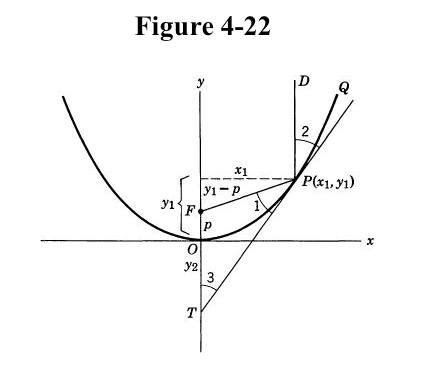
\includegraphics [scale=0.6] {Kline_4_22.png} \end{center}
Morris Kline has an alternate proof in his book \emph{Calculus}.  In the figure we need to show that angles $1$ and $2$ are equal.  By standard geometry angles $2$ and $3$ are equal, hence we need to show that angles $1$ and $3$ are equal.  We do this by showing that $FP$ is equal to $FT$.

Rather than substitute for $y = ax^2$ we just leave things in terms of $y$.  Notice that the diagram uses $p$ for the distance from the origin to the focus, and labels $P = (x_1,y_1)$.  Using Pythagoras, as indicated, the distance $FP$ is 
\[ FP = \sqrt{x_1^2 + (y_1-p)^2} \]

To get $FT$ we need to find what is labeled as $y_2$, the intercept of the tangent line with the $y$-axis.  We get this from the point-slope formula:
\[ \frac{y_1 + y_2}{x_1} = 2ax_1 \]
\[ y_1 + y_2 = 2ax_1^2 \]
But of course $y_1 = ax_1^2$ and so
\[ y_1 + y_2 = 2y_1 \]
Thus $y_1 = y_2$ and hence $FT = y_1 + p$.

Going back to $FP$, we use the same crucial fact about the focus that we relied on in the first proof, namely that $4ap = 1$ and so
\[ y_1 = ax_1^2 \]
\[ x_1^2 = 4p y_1 \]
Our previous expression was
\[ FP = \sqrt{x_1^2 + (y_1-p)^2} \]
substituting for $x_1^2$
\[ FP = \sqrt{4py_1 + (y_1-p)^2} \]
\[ = \sqrt{4py_1 + y_1^2 - 2y_1p +  p^2} \]
\[ = \sqrt{y_1^2 + 2y_1p +  p^2} \]
\[ = \sqrt{(y_1 + p)^2} \]
\[ FP = y_1 + p \]
$FT$ and $FP$ are the same length, and so the two angles are equal.  Also, we showed that $FP = y + p$, which means that every point on the parabola has the distance $y + p$ to the focus, as well as the vertical distance $y + p$ to a horizontal line a distance of $p$ below the $x$-axis and parallel to it.  This line is the directrix.


\end{document}